\documentclass[12pt]{article}

\usepackage[margin=1.0in]{geometry}
\usepackage{graphicx}

\begin{document}

\title{This is the title}
\author{Author Name}
\date{My institution}

\maketitle

\begin{abstract}
This is the abstract.
\end{abstract}

\section{Introduction}

This is the introduction.

\section{Analysis} \label{s:analysis}

\subsection{Data}

Here is the analysis.

Here's a formula: $\int_0^1 x dx+y=\pi$. More text.

\[ \int_0^1 x dx+y=\pi \]

\begin{equation}
	\int_0^1 x dx+y=\pi
	\label{eq:example}
\end{equation}

As shown by Equation \ref{eq:example} ... $1.00\pm0.02$.

\subsection{Code}

\subsubsection{Minicode}

Code!

\section{Blah}

Blah!

\begin{table}
\caption{Data table}
\centering
\begin{tabular}{l|r} \hline
Quantity & Value \\ \hline
Radius & 5 \\
Mass & 10 \\ \hline
\end{tabular}
\end{table}

\begin{figure}
\centering
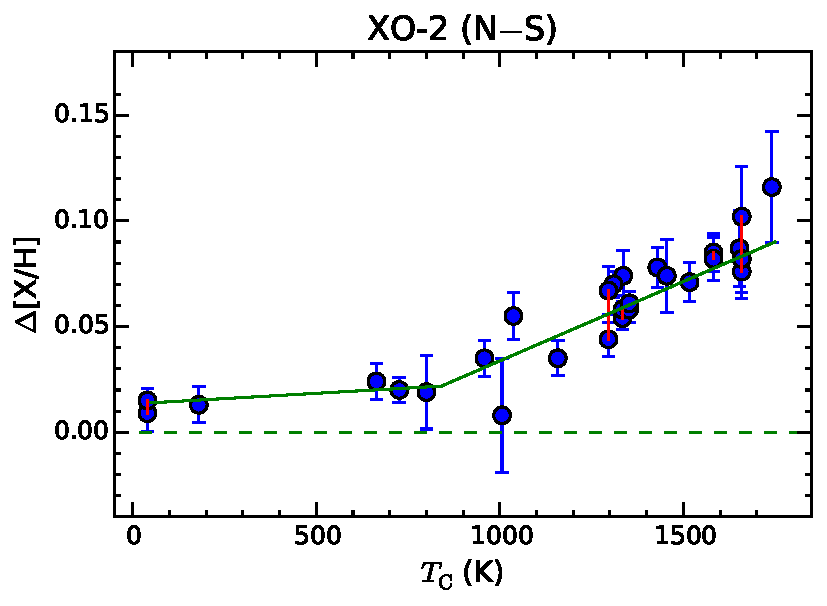
\includegraphics[width=10cm]{xo-2.pdf}
\caption{Some figure}
\end{figure}

\section{Conclusions}

Here are the conclusions. As shown in Section \ref{s:analysis}.

\end{document}
